%%%%%%%%%%%%%%%%%%%%%%%%%%%%%%%%%%%%%%%%%%%%%%%%%%%%%%%%%%%%%%%%%%%%%%%%%%%%%%%%
%2345678901234567890123456789012345678901234567890123456789012345678901234567890
%        1         2         3         4         5         6         7         8

\documentclass[letterpaper, 10 pt, conference]{ieeeconf}  % Comment this line out if you need a4paper

%\documentclass[a4paper, 10pt, conference]{ieeeconf}      % Use this line for a4 paper

\IEEEoverridecommandlockouts                              % This command is only needed if 
                                                          % you want to use the \thanks command

\overrideIEEEmargins                                      % Needed to meet printer requirements.

% See the \addtolength command later in the file to balance the column lengths
% on the last page of the document

% The following packages can be found on http:\\www.ctan.org
\usepackage{graphicx} % for pdf, bitmapped graphics files
%\usepackage{epsfig} % for postscript graphics files
%\usepackage{mathptmx} % assumes new font selection scheme installed
%\usepackage{times} % assumes new font selection scheme installed
%\usepackage{amsmath} % assumes amsmath package installed
%\usepackage{amssymb}  % assumes amsmath package installed

\title{\LARGE \bf
After You: Doorway Negotiation for Human-Robot and Robot-Robot Interaction
}


\author{Jack Thomas and Richard Vaughan$^{1}$% <-this % stops a space
\thanks{$^{1}$School of Computing Science, Simon Fraser University, 8888 University Drive, Burnaby, British Columbia, Canada.
        {\tt\small \{jackt,vaughan\}@sfu.ca}}%
}


\begin{document}



\maketitle
\thispagestyle{empty}
\pagestyle{empty}


%%%%%%%%%%%%%%%%%%%%%%%%%%%%%%%%%%%%%%%%%%%%%%%%%%%%%%%%%%%%%%%%%%%%%%%%%%%%%%%%
\begin{abstract}

We propose and test an autonomous robot behavior for socially-compliant navigation of doorways with both human and robot interlocutors. Building on previous work for ``aggressive'' interaction between robots to resolve navigation deadlocks in corridors, we demonstrate an ``assertive'' robot that negotiates right-of-way when faced with a human or other robot. The negotiation is implemented using only motion and common navigation sensors, without explicit message-passing. Our goal is for the correct agent to take priority, as decided both by time-efficiency and as judged subjectively by naive human participants. Our contribution is a practical method for doorway negotiation, and a study of human users' responses to a robot that appears to participate in existing social customs surrounding doors. Our method is evaluated with robot-robot experiments and a human-robot interaction study with non-expert users.

\end{abstract}


%%%%%%%%%%%%%%%%%%%%%%%%%%%%%%%%%%%%%%%%%%%%%%%%%%%%%%%%%%%%%%%%%%%%%%%%%%%%%%%%
\section{INTRODUCTION}

%Previously relegated to jobs considered ``dull, dirty or dangerous", robot workers are moving deeper into workplaces and public spaces alongside human beings. Amazon’s warehouses are now filled with hundreds of Kiva robots hauling goods to human coworkers, the Knightscope security robot is being tested in malls, while the self-driving car could see drivers sharing the road with the largest distributed, autonomous robot system ever built.

%This push into human environments creates new challenges, the most basic of which is how robots will navigate our socially-charged landscape.  Existing systems often avoid this problem entirely, segregating robots and humans to separate work areas or otherwise working to minimize contact between the two groups. This runs counter to the appeal of autonomous robots, whether tiny vacuums or whole transport trucks, which lies in exploiting existing human infrastructure rather than building new robot-only roads and offices.

Autonomous mobile robots are newly appearing in real world applications among humans, having previously been physically segregated to their own areas for safety. The creation of shared human-robot environments, whether in warehouses, offices or public streets, motivates us to investigate robot navigation strategies that conform with existing human social practices. One example of a common social navigation problem is resolving deadlocks at doorways. 

As seen in Figure~\ref{fig:Triptych}, the turn-taking protocol for two humans wanting to pass to opposite sides of a door is instinctive to most people. Can robots use the same behaviour to efficiently negotiate access to doors? There is no guarantee that humans will willingly integrate themselves with unfamiliar machines - in \cite{breazeal1999build}, Breazeal and Scassellati argue that to interact socially, ``humans must believe that the robot has beliefs, desires, and intentions". By this view, successfully participating in social interactions requires behaviours that promote recognition and reciprocation from human interlocutors.

With this in mind, we extended previous work on ``aggressive'' robot-robot interaction\cite{zuluaga2005reducing} for resolving deadlocks in corridors, modifying the behavior to be agnostic to whether their interlocutor is a human or another robot. Our proposed ``assertive'' system is a generalized approach to negotiating doorway interactions using only movement and distance measurements to recreate the familiar human-human social interaction.

Our intent is for this behavior to be socially compliant with humans, where one party passes through the door and the other defers to let them through. Compliance here means both that the robot respects a human's right of way when it would apply, but also that the human will reciprocate by respecting the robot's right of way in return. As well as reliably breaking the deadlock, we want the 'correct' participant to have priority, defined by the objective time-efficiency and the subjective opinion of a naive human participant. 

   \begin{figure}
      \centering
      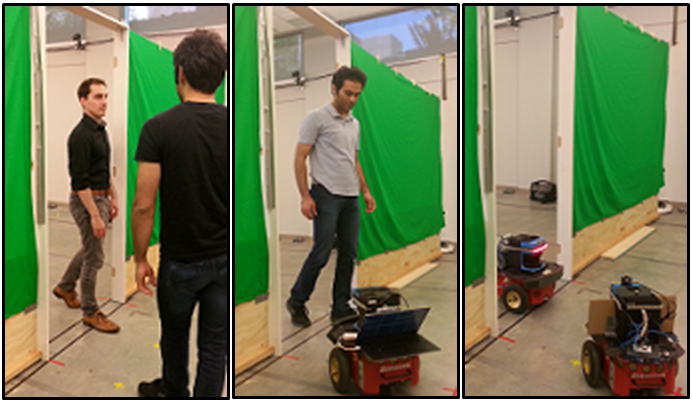
\includegraphics[scale=0.5]{Triptych.png}
      \caption{Examples of human-human, human-robot and robot-robot doorway interaction.}
      \label{fig:Triptych}
   \end{figure}

The contributions of this paper are (i) a robust doorway negotiation behavior for autonomous robots navigating shared human-robot spaces, demonstrated by real world experiments, and (ii) a non-expert user interaction study, reporting on user's perception of the robot’s behavior, and how that perception influenced navigation performance.

\section{RELATED WORK}

%Socially-compliant navigation for autonomous robots is a well-recognized interdisciplinary problem, touching on how robots navigate on their own, how humans and robots interact, and how past autonomy research has tried to use behavior to bridge that gap.

\subsection{Robot Navigation}

Navigation is one of the most frequent topics in robotics research. Most research on robot mobility focuses on the physical dynamics and geometry of getting around without considering social interaction, such as Fox et. al's Dynamic Window Approach to collision avoidance\cite{fox1997dynamic}. Other parties are often considered generically as mobile obstacles or interfering agents, with no specific human characteristics. But in crowded environments, it can help to have a more sophisticated model of other agents' mutual behaviour. The successful Reciprocal Velocity Obstacle model proposed by van den Berg et. al\cite{van2008reciprocal} dealt with mutual collision avoidance for non-communicating agents by smooth, gradual trajectories where each agent assumes the other’s cooperation in ensuring a clean pass, directly citing an interest in ``virtual human" behavior. 

This line of research has led to numerous extensions, such as Biased Reciprocal Velocity Obstacles\cite{sadat2012bravo} meant to alleviate congestion by building in more context sensitivity concerning who should defer to whom, or where Karamouzas et. al\cite{karamouzas2009predictive} turned the human-inspired model back toward humans to predict collision detection for a pedestrian simulator. Nevertheless, without explicitly designing for human interaction and studying how these behaviors are perceived in real life, these projects leave open the question of whether human-inspired necessarily equals human-compliant.


\subsection{Human-Robot Interaction (HRI)}
%IROS: Explain that the various social cost/proxemic measures tend to be continuous, aimed at passive interaction in spaces like corridors, while the doorway is more of an explicit and discrete interaction.
HRI research into compliance for human-robot behavior has already explored some parts of the problem. Kretzschmar et. al\cite{kretzschmar2016socially} produced a model for training socially-compliant trajectories directly from datasets of human observation data, in explicit recognition that navigating human environments requires adaptation to human expectations. Shiomi et. al\cite{shiomi2014towards} acknowledge in their work that solving the obstacle avoidance problem for objects is insufficient when dealing with pedestrians: models must also include the higher problem of acceptable social distances. While these proxemic-based approaches share our perspective on the needs of social HRI, their continuous and passive implementations are better suited to longer, corridor-style interactions than the explicit and discrete setting of a doorway.

There is also prior evidence that humans are willing to reciprocate with robots that attempt to participate in social customs. Park et. al\cite{park2017backchannel} found ``backchannel" signals from a listening robot in dialogue with a child would encourage that child to see the robot as more attentive to their story. For adults, a robot using recognizable gaze cues in conversation was found by Mutlu et. al\cite{mutlu2009footing} to provoke the correct social response in participants, seeing themselves as addressees or bystanders as appropriate. Mutlu argues that the social acceptance of a robot necessary for its success may hinge on their behavior and how it is perceived.

\subsection{Autonomous Robot Behavior}

One assumption made here is that multi-robot systems introduced to human environments will be autonomous and exhibiting self-regulated behaviors like the one we propose for doorway negotiation. When proposing design principles for autonomous agents\cite{pfeifer1996building}, Pfeifer described his ``fungus eaters" as ``systems capable of performing a set of tasks in the real world independently and without human intervention", able to deal with other robots, machines and humans while going about its business. These are properties we may want for robots operating in shared human-robot spaces. We speculate (but cannot prove) that robots that are autonomous or perceived as autonomous will be more readily accepted by humans into social interactions, making them potentially more efficient. This paper is part of our program to examine this hypothesis. 

%It can be difficult to find a consistent, agreed-upon definition for autonomy, but Bekey suggests\cite{c10} ``Autonomy refers to systems capable of operating in the real-world environment without any form of external control for extended periods of time." This definition is broad, but it captures the benefit we articulated earlier of integrating robots into existing human (``real world") environments who are capable of holding up their end during social interactions without direct guidance(``external control"). 

Existing research on multi-robot systems in the workplace have often had these autonomous characteristics. The STRANDS project\cite{hawes2016strands} is a sizable example where teams of robots are deployed to real office spaces for months at a time, with the stated goal of learning how to adapt and survive changes in the environment that would be fatally outside the scope of less independent robot systems. Dealing with humans around doorways is also an issue they encountered, but addressed only indirectly with passivity on the part of the robot, where humans near doors are treated as obstacles rather than potential interaction partners.

These autonomous characteristics will also be present in the systems coming to share human spaces that we mentioned earlier. The self-driving car is the most obvious example, referred to almost interchangeably as the autonomous car in the popular press\cite{EconomistAuto}. The conditions involved in driving – wide open spaces, large numbers of human and robot agents, the need to act quickly without guidance in network-denied environments – suit an autonomous approach.


\section{SYSTEM OUTLINE}

The problem our behavior solves is for an autonomous robot to reliably pass through a doorway when an interlocutor on the other side (whether another robot or a human) is trying to do the same, such that each blocks the path of the other. Our robot must decide either to make way for the opponent or take the right of way if the opponent offers it, as sketched in Figure~\ref{fig:Wireframe}. Since our interlocutor may be a human or human-controlled, we cannot assume the other party shares our robot’s programming or can communicate over the same network, so the interaction must be mediated through local sensor data alone, and by direct interaction. We build on previous related work for resolving robot-robot spatial competition in tight corridors under similar constraints.

    \begin{figure}
      \centering
      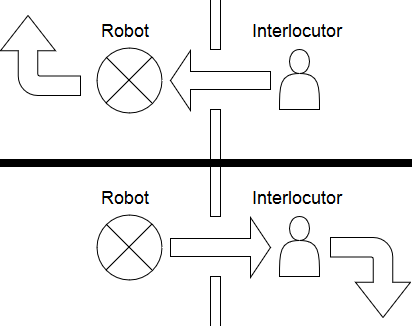
\includegraphics[width=0.6\columnwidth]{wireframe.png}
      \caption{Sketch of outcomes for a doorway negotiation behavior. One party retreats and makes room for the other to advance. Which outcome is `correct' can be determined by some combination of an objective efficiency measure and the subjective opinion of a human interlocutor.}
      \label{fig:Wireframe}
   \end{figure}

\subsection{Aggressive Displays for Robot-Robot Corridor Negotiation}

In Zuluaga et al \cite{zuluaga2005reducing}, autonomous robots who approached one another in a corridor and found their paths mutually blocked would engage in a brief interaction to determine who would make way. Upon detecting each other, both robots would stop and begin backing away until one robot achieves their desired ``safe distance'' from the opponent. The safe distance is inversely proportional to the robot's ``aggression'': a simple scalar value.

On reaching its safe distance, the more aggressive robot would become ``brave" and start advancing toward the other robot, who would no longer be able to achieve their own safe distance until backing out of the corridor completely and allowing the aggressor to pass. A flowchart for this behavior can be seen in Figure~\ref{fig:Aggressive}.
 
    \begin{figure}
      \centering
      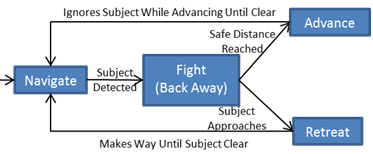
\includegraphics{aggressive_behavior.png}
      \caption{Outline of the Aggression System for Robot-Robot Corridor Interaction}
      \label{fig:Aggressive}
   \end{figure}
 
A robot's aggression value is best decided dynamically by encoding the cost the robot would experience if it ``lost'' the contest. Alternatively it can be a constant: if each robot has a different constant aggression, a dominance hierarchy is obtained.
 
This system took deliberate inspiration from aggression displays in nature, used to assert dominance or divide resources. It was speculated at the time that it would also be compatible with humans, but this was not explicitly considered during the design process or evaluated with users. 


\subsection{Assertive Displays for Robot-Human and Robot-Robot Doorway Negotiation}
%IROS: explain a little more why we need the modification, and why we didn't bother to test the aggressive method
We modify the aggressive display method to work in doorways rather than corridors, and with the specific needs of human-compliant interaction in mind. To wit, we adopt the term ``assertive'' instead of ``aggressive'' to  represent participating in polite human social etiquette but maintaining a willingness to assert the robot’s own right of way, and avoid the negative valence of `aggression'. We do not want the robot to always give way to humans, since this may not be the most objectively efficient ordering \cite{zuluaga2005reducing}.

%IROS: Moved the specific value of the half-step to the parameter discussion to avoid giving specific implementation details in the high-level algorithm explanation.

\textit{Modification 1}:  When a robot finds its path blocked, it backs up a half-step and stops, to signal it has acknowledged the impasse and is waiting for an interaction to resolve it. The motivation for this design over the previous immediate retreat is that we do not want to signal immediate deference to a human user. The pause near the door is intended to signal the robot's desire to get through the door as soon as possible.

\textit{Modification 2}: Instead of signalling aggression/assertiveness by distance, we use waiting time. Instead of retreating further the robot waits, with a more assertive robot waiting a shorter time before trying to advance. While waiting, when a robot detects an advancing interlocutor it backs up and attempts to move out of the way by turning to the side, as shown in Figure~\ref{fig:Wireframe}.


\textit{Modification 3}: We must also address cases where interlocutors do not move if approached, or both parties decide to advance simultaneously. We use a minimum distance which, if breached by the interlocutor while the robot is advancing, will cause the robot to stop. If the interlocutor backs away then the robot will resume advancing, otherwise the robot will wait a time inversely proportionate to the time they waited before advancing (so that a more assertive robot will wait longer for an intransigent subject to move), before switching to retreating in hopes that the interlocutor will finally clear the way. A subject that cannot or will not clear the blocked doorway is an obstacle rather than an interaction partner, and should be handled by another means beyond our scope. 
 
    \begin{figure}
      \centering
      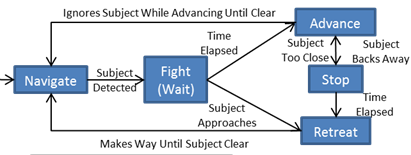
\includegraphics{assertive_behavior.png}
      \caption{Outline of the Assertive System for Negotiated Doorway Interaction}
      \label{fig:Assertive}
   \end{figure}


The high-level interaction behavior flowchart can be seen in Figure~\ref{fig:Assertive}, independent of implementation details. As with the previous aggression system, the behaviour is meant to be generalizable to any mobile robot platform with the means to judge distance and discern subjects from the environment. 

%IROS: Discussing how this situation is narrowly defined and how previous aggression research already explored extensions, but the core behaviour is a real interaction case worth evaluating first.

It is worth acknowledging that the doorway interaction described here is strictly defined, and has not been extended to cases such as multiple agents approaching a door from the same side. Existing research on aggression has explored some of these, such as the case where a lone robot on one side of a door should yield to an opposing group[REF]. The isolated case of a head-on one-on-one interaction is nevertheless a real use case that also forms the basis of these more complicated scenarios, and warrants evaluating first for sake of clarity.

%Various extensions are easy to imagine, but for clarity we evaluate this simple base system.

\section{EXPERIMENT AND STUDY}

Our behavior is intended as a socially compliant means to solve navigation deadlocks around doors. Socially compliant here means that humans can recognize the robot's signals of intent and cooperate with it to mutual benefit. In order to test this claim, we have three hypotheses that we evaluated through a robot-robot experiment and human-robot study:

\textbf{H1)} The assertive behavior resolves doorway navigation deadlocks for both human and robot agents.

\textbf{H2)} Overall performance of the behavior will be improved if humans respect the robot's right of way.

\textbf{H3)} Respecting the robot's right of way will correlate with recognizing their participation in a human social interaction.


\subsection{Setup}

Testing was divided into two phases: one set of experimental robot-robot interactions, and one user study of human-robot interactions. The environment, robots, software and parameters were identical in both scenarios.

The test environment for all experiments is shown in Figure~\ref{fig:Example}: a lab with a wall erected to divide the test space into two smaller rooms and with an open, standard-sized (97cm wide) doorway centered in it. Subjects in the smaller room would begin 2m from the door, while subjects in the larger room would begin 4m away. This ensured the closer party in each interaction should have right of way by arriving at the door first, as we would expect from two humans in this setting (all else being equal).

%IROS: I further explained the choice of navigation and detection algorithms, and tried to justify our permissive detections by the needs of the study. I also mentioned "for safety" on the speed in hopes of mollifying questions about why that speed was chosen.

Robots were Pioneer 3DXs, mounted with SICK LMS200 forward-facing laser range finders. Localization was achieved through a known map and AMCL[ref], while standard navigation was provided by the standard ROS Navigation stack[ref]. Human detection was achieved through comparisons with the map for any unmapped obstacles, a permissive strategy as the cost of false negatives during the study would be high. The Pioneers used rear-mounted sonar rangers while retreating to avoid collisions. They had a top speed of 0.5m/s for participant safety and stood 0.74m tall due to a paperwork-storing boxy, which gave them enough physical size to make stepping over them impractical.

%IROS: Parameter setting discussion
The parameters for the assertive behaviour include a 2m forward arc detection range for interaction, a 0.35m emergency stop distance, a two-second wait time when robots are being assertive and an eight-second wait otherwise. The half-step backward after detecting a human was set to 0.15m. These parameters were derived through informal testing beforehand rather than rigorous optimization, as a system requiring intense fine-tuning to perform adequately

A strip of LEDs were mounted on the front of the Pioneer and would turn on when the behavior was active and turn off after arriving at its destination. These lights were green while traveling from the larger room to the smaller one and red on the return journey, which also corresponded to lower and higher assertiveness respectively, following our assumption about right of way. This very basic feedback was included to see whether participants would correlate the color of the light with the assertiveness of the robot.

\subsection{Robot-Robot Experiment}

Each robot was set at their respective starting points either side of the doorway. At the beginning of each trial, the further robot would be given the instruction to drive to the other robot’s starting point, and after approximately one second the closer robot would receive the same instruction. This ensured the robot starting inside the smaller room would most likely reach the doorway first (with some variation on their exact meeting point) and was given the higher ``assertiveness" variable to reflect their expected right of way.

The desired outcome for each trial was that the more assertive, nearer robot would win the ensuing contest and have the other robot retreat until it could pass, whereupon the other robot would resume and finish its journey. Once both robots had reached their destinations, they would swap assertiveness values and goals and repeat the process. This was repeated 49 times, with the outcomes, interaction times and errors or other incidents recorded. 

\subsubsection{Results}

Of the 49 trials, 5 were discarded due to irrelevant navigational errors due to the commodity motion planner. Of the remaining 44 valid trails, 40 trials resolved the doorway contention in a single interaction. In the remaining four cases, each robot first believed the other robot was approaching them and both retreated simultaneously, but they correctly resolved the interaction on the second attempt. All 44 trials ended with the intended robot winning the interaction and both arriving at their desired destinations.

These trials show that the assertive strategy can robustly resolve robot-robot doorway contention. 

\subsection{Human-Robot Study}
%IROS: Tried to imply age range with "students" without hard numbers
20 participants were recruited from the general population of Simon Fraser University, predominantly students, including 8 women and 12 men. They were not compensated for their assistance.

     \begin{figure}
      \centering
      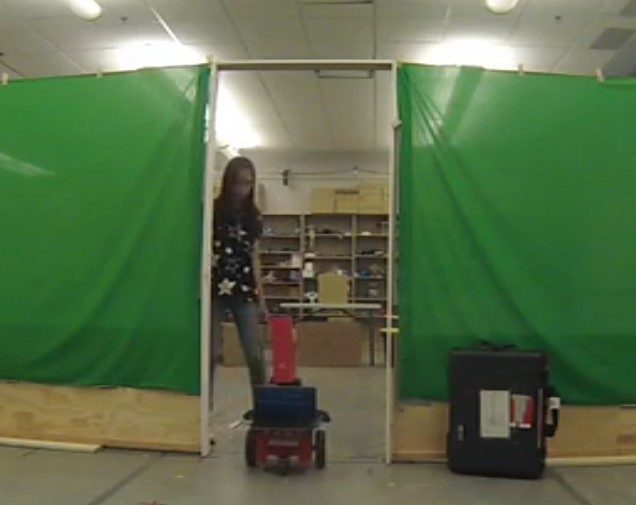
\includegraphics[width=\columnwidth]{test_example.png}
      \caption{A study participant deferring to the robot's right of way}
      \label{fig:Example}
   \end{figure}

Each participant was brought to the test environment and seated across from the test conductor in the smaller room, passing by the robot prepared for the experiment in the larger room. Every trial had the participant drop a document in a box in the larger room while the robot entered the smaller room to pick up some excess paperwork from the test conductor, then had the participant and robot return to their starting points. This created two interactions per trial, where we intended the human to have the right of way in the first part and the robot in the second, because they arrived at the door slightly earlier than their opponent. An example of a participant completing the study can be seen in Figure~\ref{fig:Example}. Each participant completed five trials:

\textbf{1) First Reaction Trial:} Without being informed as to the details of the experiment, the participant was asked to drop their signed consent form in a box on a table in the larger room, while the robot would be called in to collect the reusable part of the form. The participant apparently incidentally interacted with the robot around the door as a result, and then again on their return journey. The participant was then informed that these incidental interactions were actually one of the trials, and the intent of the study was to examine their interactions with the robot around the doorway.

\textbf{2) Teleoperation Trial:} The participant was informed that the test conductor will take direct control of the robot via a controller, but to otherwise focus on the robot when deciding when to pass. 

\textbf{3) Full System Trial:} The participant was informed the full autonomous system would now be active and the test conductor would no longer be in control of the robot.

\textbf{4) Directed Behavior Trial:} For the first interaction, the participant was instructed to treat themselves as having absolute priority over the robot, and that the robot should defer to them. For the second, they were told to now treat the robot as having full priority, and that they should defer to it.
%IROS: Clarified participants are not instructed to follow the system's intentions
\textbf{5) Full Explanation Trial:} Before beginning the trial, the test conductor fully explained how the system worked to the participant, without instructing them on whether or not to obey it.%answering all questions until they were satisfied.

After each trial, the participant was given a survey to complete. These surveys contained four 5-point Likert Scale questions on the participant’s perception of the robot and the interaction during that trial. The survey questions were presented as statements with a scale ranging from strongly agree to strongly disagree, and are listed in Table 1.

\begin{table}[h]
\caption{Post-Trial Survey Questions}
\label{survey_questions}
\begin{center}
\begin{tabular}{|c|}
\hline
1) The robot’s intentions appeared clear.\\
\hline
2) The robot appeared to understand my intentions.\\
\hline
3) Our interaction went as smoothly as \\
it would have with another human.\\
\hline
4) The interaction was satisfactory overall.\\
\hline
\end{tabular}
\end{center}
\end{table}

Each survey also included a field for the participant to write their account of what had happened during the trial and another field for additional comments. This form was what the participant would drop off in the box in the large room for each trial.

Once all five trials were complete, a post-test questionnaire was administered by the test conductor, who transcribed the participant’s spoken responses. These questions are listed in Table 2.

\begin{table}[h]
\caption{Post-Test Questionnaire}
\label{questionnaire_questions}
\begin{center}
\begin{tabular}{|c|}
\hline
1) If or when you chose to press the robot, what \\
informed that decision in terms of signals you \\
were getting from the robot and your own motivations?\\
\hline
2) What about when you chose to defer to the robot?\\
\hline
3) In which trial do you think the interaction \\
worked best, in terms of getting where you \\
wanted to go and communicating between you and \\
the robot?\\
\hline
4) How would you compare these interactions to \\
those you have with other humans around doors?\\
\hline
5) What other behavior would you like to see from the robot? \\
What other feedback?\\
\hline
6) Any additional questions or observations.\\
\hline
\end{tabular}
\end{center}
\end{table}

\subsection{Results}

     \begin{figure}
      \centering
      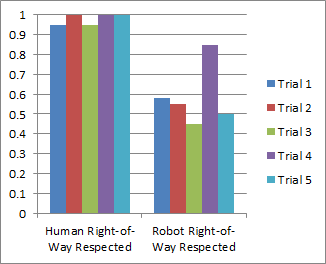
\includegraphics{outcomes.png}
      \caption{Outcomes Of Human-Robot Study Interactions Per Trial}
      \label{fig:Outcomes}
   \end{figure}

\textbf{1) Outcome:} The results for the human-robot interaction study are in Figure~\ref{fig:Outcomes}, showing the proportion of times the 'correct' right of way was respected. The near-unanimous respect for the human's right of way in all trials when the participant was closest to the door demonstrated the interaction completed successfully without insisting on its right of way inappropriately. Analyzing the second half of each trial revealed four discrete categories of participant: 

A) Those who would never respect the robot's right of way, sometimes even in trial 4 when specifically asked to. 

B) Those who did not respect the robot's right of way until the last trial then changed their behavior. 

C) Those who respected the robot's right of way until the last trial then changed their behavior. 

D) Those who always respected the robot's right of way. 

Our 20 participants were divided relatively evenly between these four categories, with five type A, four type B, five type C and six type D.
 %IROS: Clarified end-of-interaction qualifier, modified discussion to be about combined figure
\textbf{2) Timing:} Our data from both the robot-robot experiment and human-robot study is collected in Figure~\ref{fig:Trial_Interaction} for time both subjects spent interacting during each trial and total time until both subjects reached their destinations, both with standard deviation error bars. Interaction time was measured from the point in each video that the robot reacted to the human's presence to the point that both they and the human are once again centered in their respective lanes, and represents a subset of the total time for each trial. In each trial, part 1 was the interaction where the human had right of way, while the robot had right of way in part 2. For context, one Pioneer making the 6m journey from one starting point to the other uninterrupted takes approximately 12 seconds. The robot-robot trial times are included for comparison.  
 %IROS: Replacing with one combined figure

%       \begin{figure}
 %     \centering
  %    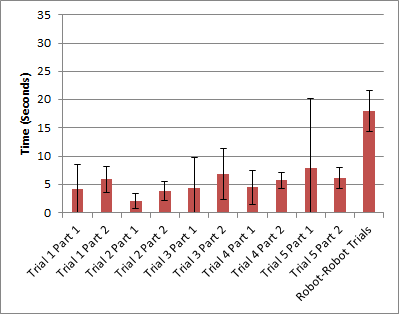
\includegraphics{interaction_length.png}
   %   \caption{Average Length Of Each Interaction In Each Trial}
    %  \label{fig:Interaction}
   %\end{figure}


%     \begin{figure}
 %     \centering
  %    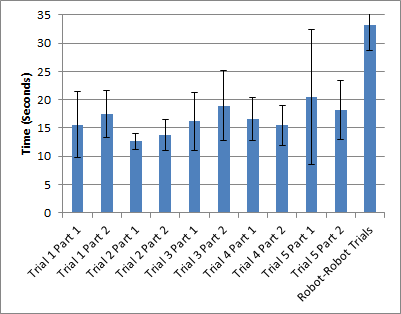
\includegraphics{trial_length.png}
   %   \caption{Average Length Of Each Trial}
    %  \label{fig:Trial}
   %\end{figure}
   
        \begin{figure}
      \centering
      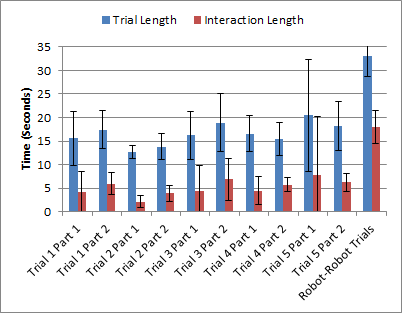
\includegraphics{Interaction_Trial.png}
      \caption{Average Length Of Each Trial And Interaction}
      \label{fig:Trial_Interaction}
   \end{figure}

The robot-robot behavior is much slower than any human-robot behavior measured. Thus the human behaviour made a positive contribution to system performance compared to robot-only system. This might be largely explained by  humans moving faster than our robots. However, the human-robot interactions observed in the four non-teleoperated trials are only marginally slower than the interaction in the second trial, where a human is controlling the robot. This suggests that in terms of efficiency, our behavior may already be operating close to what might be possible for our robot platform. Human interlocutors were able to compensate for the relatively cautious speed of the robot regardless of how it was being controlled. 

%IROS: Significance testing done to aggregate results of respecting vs. not-respecting behaviour, with a t-test significance of +99%
If we break down these time results according to our four participant behavior categories, seen in Figure~\ref{fig:Respect}, we found that participants who did not respect the robot's right of way had higher trial times than those who did across all trials. This is supported via the aggregate trial times of all interactions where the robot was respected versus all interactions where it was not, resulting in averages of 14.3 and 19.6 seconds respectively, with a t-test confidence greater than 99\%.  This reflects that while going out of turn might benefit the human individually, it degrades the throughput of the overall environment. 

     \begin{figure}
      \centering
      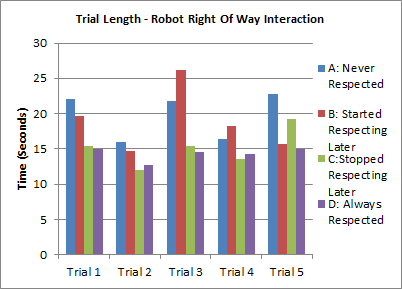
\includegraphics{Robot_right.png}
      \caption{Average Trial Length While Robot Had Right Of Way Per Participant Type}
      \label{fig:Respect}
   \end{figure}

\textbf{3) Surveys:} The data from the four Likert-scale questions on the post-trial surveys is collected in Figure~\ref{fig:Questionnaire}, with standard deviation error bars. The interaction was mainly positively received in each trial, but the higher time for Q3 during trial 2 may suggest that knowing a human operator was controlling the robot was relevant to some participants. Similarly, some difficulty reading the robot's intentions in the very first interaction could have led to the relatively low Q1 score during trial 1.
 
     \begin{figure*}
      \centering
      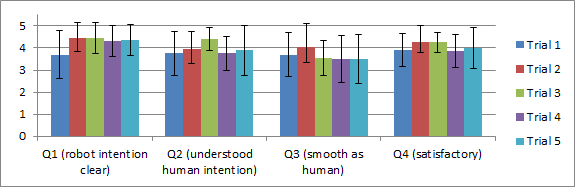
\includegraphics[width=\textwidth]{Questionnaire.png}
      \caption{Average Survey Score Per Trial Per Question }
      \label{fig:Questionnaire}
   \end{figure*}
 
Breaking down the scores according to our four participant categories did not produce a clear correlation between respecting the robot's right of way and a positive survey result. In fact, it was the type C and D participants in the first trial that gave low ratings for clear intentions and satisfaction. A participant who found they could make the robot back down in every confrontation may rate the interaction as satisfying as one who chose to respect the robot's right of way every time. These scores alone are not enough to distinguish different perceptions of the robot's behavior.

\textbf{4) Post-Test Questionnaire:} The questionnaire data was mostly qualitative, with the exception of question three where the participant gave their preferred trial. The overall results for this question are presented in Table 3 (with one abstention).

\begin{table}[h]
\caption{Number of Participants who Preferred Each Trial }
\label{Preferences}
\begin{center}
\begin{tabular}{|c||c|}
\hline
Trial One & 3\\
\hline
Trial Two & 4\\
\hline
Trial Three & 5\\
\hline
Trial Four & 3\\
\hline
Trial Five & 4\\
\hline
\end{tabular}
\end{center}
\end{table}

Breaking down these preferences by our four participant behavior categories saw no notable trend. Instead we observed common justifications shared by participants who chose the same trial as their preference. All three participants who chose trial 4 cited that they preferred the decision on whether to defer to the robot or not be taken out of their hands, and similarly those who chose trial 2 mostly cited the speed of the interaction when the robot was being teleoperated. Participants who chose one of trials 1, 3 or 5 highlighted understanding the robot's intentions and the sense that it understood theirs, sometimes even directly declaring the humanlike characteristics of the behavior.

%The first two questions on the post-test questionnaire directly address why the participant would choose to advance or make way. Here we saw a difference between those who did and did not respect the robot's right of way, with those who did not predominantly phrasing their explanations in terms of efficiency - the robot was too slow, blocking their way. A smaller number believed they always had right of way, or that hesitation was an invitation to take the initiative. Some were curious what the robot would do if approached, and a few mentioned concerns that it might collide with them.

%By contrast, those who respected the robot's right of way often acknowledged that right as their reason. One mentioned buying into the premise of the study, assuming the robot might be carrying out some important work, and another suggested coworkers should be ``compatible". Curiosity was brought up, but also caution, concerned that they might damage or break the robot.

The first two questions on the post-test questionnaire directly address why the participant would choose to advance or defer. Lack of space forbids reproducing these responses verbatim, so they were codified according to one of seven types, and the 20 answers to each question are presented in Tables 4 and 5, grouped according to participant behaviour. The seven observed types of responses were:

\textit{Efficiency:} For the fastest resolution.

\textit{Right:} Acknowledged right of way.

\textit{Curious:} To see what would happen.

\textit{Safety:} To protect themselves or the robot.

\textit{Never:} Wouldn't do this.

\textit{Test:} Believed it was required by the test.

\textit{Learned:} In response to learning how the system worked in trial 5.

\begin{table}[h]
\caption{Cause For Advancing Toward Robot}
\label{Advance}
\begin{center}
\begin{tabular}{|c||c||c||c|}
\hline
\textbf{A} & \textbf{B} & \textbf{C} & \textbf{D}\\
\hline
Efficiency & Right & Learned & Safety\\
\hline
Efficiency & Curious/Test & Learned & Efficiency\\
\hline
Right & Efficiency & Curious & Right\\
\hline
Curious & Test & Efficiency & Efficiency\\
\hline
Right & & Curious & Curious\\
\hline
 & & & Right\\
\hline
\end{tabular}
\end{center}
\end{table}

\begin{table}[h]
\caption{Cause For Deferring To Robot}
\label{Defer}
\begin{center}
\begin{tabular}{|c||c||c||c|}
\hline
\textbf{A} & \textbf{B} & \textbf{C} & \textbf{D}\\
\hline
Safety & Safety & Right & Right\\
\hline
Right & Safety & Curious & Safety\\
\hline
Curious & Right & Curious & Right\\
\hline
Curious & Right & Right & Right\\
\hline
Never & & Right & Safety\\
\hline
 & & & Right\\
\hline
\end{tabular}
\end{center}
\end{table}

The number of participants who acknowledged the robot's right of way went from one among those who never deferred to four among those who always did. One type D participant mentioned buying into the premise of the study, assuming the robot might be carrying out some important work, and another suggested coworkers should be ``compatible". The difference could also be seen in the safety response, where type D participants were worried they could damage the robot. By contrast, the type A participants imagined deferring only out of curiosity, to protect themselves, or in one case not at all, with one at least conceding the idea of respecting the robot's right of way.

There were fewer differences between participants when comparing the interaction to those with other humans in the fourth question. The most common observation was that the robot was slower and less maneuverable than a human, and while some suggested the robot acted in a human-like manner it was couched as ``similar", yet still different.

Both the fifth question and the interaction accounts from the surveys produced a number of small implementation suggestions to smooth the interaction. Several participants noted that a human would know which direction to back up in order to clear the way faster, and others suggested that a human would speed up after noticing someone was already getting out of their way to minimize that person's delay. A few noted the Pioneer's wheels kept it from stepping briskly to the side the way a human might. Three participants described what was effectively a Reciprocal Velocity Obstacle interaction, where the robot cooperates at distance for a closer pass rather than one being forced to stop and back away from the other. 

\section{DISCUSSION}

\subsection{Hypotheses}

Our first hypothesis was that our behavior would resolve doorway navigation deadlocks, and in terms of both parties arriving at their destinations without incident that was the case in virtually all trials (a few unrelated navigation errors notwithstanding). Defined more narrowly, we found that our behavior executed as intended where the party with right of way was allowed to pass first in a single interaction in almost all robot-robot trials and those human-robot interactions where the human had right of way. 

While most participants ignored the robot's right of way during at least one trial, 85\% could still complete the interaction as intended when asked to do so in trial 4. With that trial as a baseline, we can say the behavior succeeded in resolving doorway deadlocks for both humans and robots, contingent on the cooperation of the human.

Our second hypothesis concerned whether respecting objective right of way increased overall performance, and average trial times showed  improvement for those who did. However, this metric places the throughput of a shared human-robot environment above the personal benefit to the individual human of reaching their destination as soon as possible, a perspective the human may not share. This is not a problem unique to human-robot interaction, behaving socially could produce better outcomes for humanity in general over being anti-social, but hinges on the cooperation of all participants.

This leads into our third hypothesis on whether those who respected the robot's right of way recognized the robot as participating in a social interaction. Gaining recognition is not something unique between humans, as participants were no more likely to respect the robot's right of way while it was being teleoperated than they were while it was controlled by our system. Few participants preferred the human-operated trial and none of those cited the human as the cause, while the ``smooth as human" survey result for the teleoperation trial was only marginally higher than the rest.

The suggestions from the questionnaire and accounts on how to enhance the interaction demonstrated that participants were actually looking for more reciprocation from the robot for the social courtesies they extended, even if they did not recognize the robot's right of way themselves. For those who did, they cast their decision to defer in terms of right and mutual concern. This contrasts with the accounts of those that did not, who broadly ignored the robot's rights in favor of their own or simple efficiency.

\subsection{Limitations}
%IROS:Further elucidated on how other environments and more agents could be explored in the future, and previous aggression work could be adapted.
As this method is meant to generalize to any ground robot, it should be tested beyond the platform, parameters, detection methods and other particulars chosen here. It is likely that the exact form factor of the robot chosen had a significant effect on user perception of the behavior, and some performance shortfalls might be mitigated with more responsive movements and detections. 

The simple green/red LED signals also provoked very little participant interest. There was no evidence that participants distinguished between different levels of assertiveness or associated them with the different colors. Instead, several participants expressed a desire in the questionnaire for more indications of a robot’s intended action and direction, whether through subtle body language or explicit flashing lights, and a few thought the robot should state its intentions aloud. 

\subsection{Future Work}
%IROS: Make reference to cultural factors
While we saw evidence that our system did provoke reciprocation from some participants, the large proportion who did not respect the robot's right of way shows that work remains in achieving acceptance. Establishing that perceiving the robot as participating in social interactions could promote compliance in users provides a goal, while participant feedback highlighted additional behaviors to improve the experience. Further studies with larger or more diverse pools of participants could further refine this feedback to account for specific cultural factors that differ between populations[ref].

%IROS: I propose cutting this paragraph since it sort of restates what's already said in limitations, that if we had better detection methods and platform capabilities then the system might work better.
%Improving the platform’s sensor capabilities would allow the system to integrate more nuanced information when deciding when to act, like gestures or speech. Though these capabilities were deliberately excluded to focus attention on the performance of the behavior, participant feedback emphasized the importance of picking up smaller multi-modal cues to make the interaction more natural.

One avenue of exploration was revealed by accounts of the fifth trial. In some cases, particularly the type C participants who stopped respecting the robot's right of way in the last trial, hearing an explanation of how the behavior worked appeared to turn it into a mere mechanism rather than a social interaction. Several chose to play with the robot, deliberately triggering a fight over and over to see if it would respond as predicted. Perhaps behavior development strategies that obscure the inner workings of a system, like machine learning, could improve human perception.

\section{CONCLUSION}

This paper proposed an ``assertive" approach for robots to negotiate deadlocks at doors in a way compatible with both robots and humans. We tested our behavior with an experiment and a study, and found it resolved both robot-robot and human-robot impasses. Further, by examining what effect cooperation by humans had on performance and what provoked compliance, we found evidence that recognition of robot social participation by humans may be an important part of successful navigation.

Our system contributes to the growing effort to integrate robots into human environments. If we want to advance robots further into the public sphere where humans will be asked to share space with them, we should consider what the necessary conditions are for achieving efficient and inoffensive coexistence.

\section*{ACKNOWLEDGMENT}

The authors would like to thank our participants for their assistance. This work was funded by the NSERC Field Robotics Network (NCFRN) of Canada.


\bibliographystyle{IEEEtran}
\bibliography{cite}

\end{document}
